\phantomsection
\chapter[Training a Computer to Classify White Blood Cells]{Training a Computer to Classify White Blood Cells\chapsubhead{Phillip Compeau}}
\label{chapter:white_blood_cells}
\renewcommand{\chaptertitle}{Training a Computer to Classify White Blood Cells}
\addcontentsline{cc}{chapter}{Chapter \thechapter} % Adds chapter number to table of contents


%\clearpage \null
%\thispagestyle{empty}
%\AddToShipoutPictureBG*{% Add picture to current page
%  \AtStockLowerLeft{% Add picture to lower-left corner of paper stock
%    \includegraphics[width=\stockwidth]{images/CMYK_ed3/cover/alignment_final}}
%}
%\addtocounter{page}{-1}
%\clearpage

\FloatBarrier

\section{Introduction: How Are Blood Cells Counted?}
\label{sec:introduction}
\phantomsection

Your doctor sometimes counts your blood cells to ensure that they are within healthy ranges as part of a complete blood count. Blood cells consist of \textdef{red blood cells (RBCs)}{red blood cells (RBCs)}{FILL IN}, which transport oxygen via the hemoglobin protein, and \textdef{white blood cells (WBCs)}{white blood cells (WBCs)}{FILL IN}, which help identify and attack foreign cells as part of your immune system.

The classic device used for counting blood cells is the \textdef{hemocytometer}{hemocytometer}{FILL IN}. In this device, a technician filters a small amount of blood onto a gridded slide and then counts the number of cells of each type in the squares on the grid. As a result, the technician can estimate the number of each type of cell per volume of blood.

\texttt{NEED FIGURE HERE -- TO REPLACE VIDEO}

\begin{qbox}[%
Why might the size of the blood sample influence the estimate of blood cell count?
]\end{qbox}

If the hemocytometer seems old-fashioned, you are not wrong; it was invented by Louis-Charles Malassez 150 years ago. To reduce the human error inherent in using this device, what if we train a computer to count blood cells for us?

We will focus specifically on WBCs. A low WBC count may indicate a host of diseases that leave the immune system susceptible to attack; a high WBC count may indicate that an infection is present, or that a disease like leukemia has caused overproduction of WBCs.

WBCs divide into families based on their structure and function, and some diseases may cause an abnormally low or high count of a specific WBC classes. We therefore wish not only to identify WBCs in cellular images but also to \textdef{classify}{classify}{FILL IN} WBCs into their appropriate types.

We will work with a publicly available dataset (hosted at \url{https://github.com/Shenggan/BCCD_Dataset}) containing blood cell images that depict both RBCs and WBCs, as shown in \autoref{fig:three_families}. The cells have been applied with a stain in which a red-orange dye bonds to hemoglobin and a blue dye bonds to DNA and RNA. The red-orange dye will make the RBCs (which do not have DNA or RNA) look red, and the blue dye will make the WBC nuclei look purple.

\autoref{fig:three_families} also illustrates the three main families of WBCs: \textdef{granulocytes}{granulocytes}{FILL IN}, \textdef{lymphocytes}{lymphocytes}{FILL IN}, and \textdef{monocytes}{monocytes}{}.  Granulocytes have a \textdef{multilobular nucleus}{multilobular nucleus}{FILL IN}, which consists of several round “lobes” that are linked by thin strands of nuclear material. Monocyte and lymphocyte nuclei only have a single lobe, but the shapes of the nuclei are quite different: lymphocyte nuclei tend to have a more rounded shape (taking up a greater fraction of the cell’s volume), whereas monocyte nuclei have a more irregular shape.

\begin{figure}[p]
\centering
\tabcolsep = 2.5em
\mySfFamily
\begin{tabular}{c c c}
\end{tabular}
\caption{Three images from the blood cell image dataset showing three types of WBCs. In our dataset, these cells correspond to image IDs 3, 15, and 20. (Left) A specific subtype of granulocyte called a neutrophil, illustrating the multilobular structure of this WBC family. (Center) A monocyte with a single, irregularly-shaped nucleus. (Right) A lymphocyte with a small, round nucleus.}
\label{fig:alignment_game}
\end{figure}

In this module, our goal is twofold. First, can we excise, or \textdef{segment}{segment}{FILL IN}, WBCs from these cellular images? Second, can we train a computer to classify WBCs by family? To perform these tasks, we will enlist CellOrganizer (\url{http://www.cellorganizer.org}), a powerful software resource that can perform a wide variety of automated analyses on cellular images.

When you look at the cells in the figure above, you may think that our two tasks will be easy. Identifying WBCs only requires identifying the large purplish regions, and classifying them is just a matter of categorizing them according to the differences in shape that we described above. Yet even after decades of research into computer vision, researchers struggle to attain the precision of the human eye.

\FloatBarrier
\phantomsection

\section{Segmenting White Blood Cell Images}
\label{sec:segmenting_white_blood_cell_images}
\phantomsection
\subsection{Image segmentation requires a tailored approach}


We begin our work by discussing how to segment WBCs from an image of blood cells like the one in the figure below, reproduced from the introduction.

BETTER CITATION OF NEUTROPHIL IMAGE 3

Researchers have developed many algorithms for cellular image segmentation, but no single approach can be used in all contexts. We therefore will identify the key attributes that make this dataset special and then use these features to develop our own segmentation algorithm.

We ask what makes the WBC nucleus so easy for a human to spot in the above blood cell. You may be screaming, ``It is dark blue! How hard could it be?'' But to train a computer to segment images by color, we should first understand how the computer represents color in images.

\FloatBarrier
\phantomsection
\subsection{The RGB color model}

In the \textdef{RGB color model}{RGM color model}{FILL IN}, every rectangular pixel on a computer screen receives a solid color formed as a mixture of the three primary colors of light: red, green, and blue (hence the acronym ``RGB''). The amount of each color in a pixel is expressed as an integer between 0 and 255, inclusively, where larger integers correspond to larger amounts of the color.

A few colors are shown in \autoref{fig:RGB_color_chart} along with their RGB equivalents; for example, magenta corresponds to equal parts red and blue. Note that a color like (128, 0, 0) contains only red but appears duskier than (256, 0, 0) because the red has not been “turned on” fully.

\begin{figure}[h]
\centering
\mySfFamily
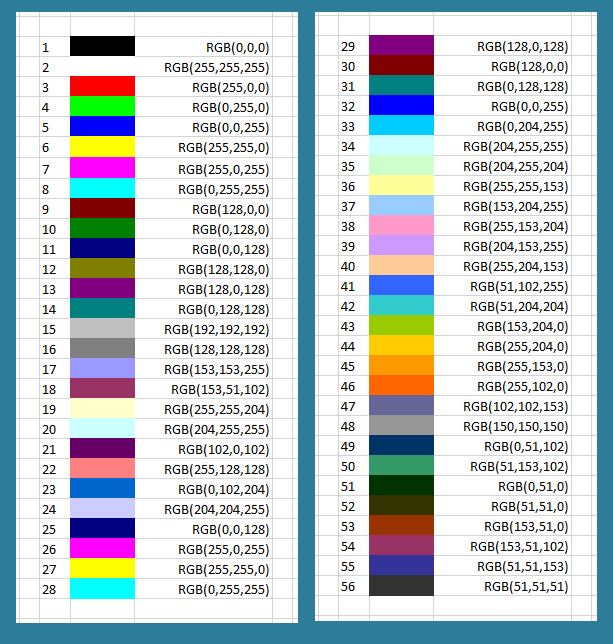
\includegraphics[width = 0.444\textwidth]{../images/RGB_color_chart.png}
\caption{A collection of colors along with their RGB codes. This table corresponds to mixing colors of light instead of pigment, which causes some non-intuitive effects; for example, yellow is formed by mixing equal parts red and green. The last six colors appear muted because they only receive half of a given color value compared to a color that receives 256 units. If all three colors are mixed in equal proportions, then we obtain a color on the gray scale between white (maximum amount of all three colors) and black (no color). Source: https://excelatfinance.com/xlf/xlf-colors-1.php; Excel at Finance.}
\label{fig:RGB_color_chart}
\end{figure}

The RGB model gives us an idea for finding a WBC nucleus. If we scan through the pixels in a blood cell image, we can “turn off” any pixels whose RGB color values are not sufficiently blue.

\begin{qbox}[%
You can find a color picker in \texttt{Utilities > Digital Color Meter} (Mac OS X) or by using ShareX for Windows. Open your color picker, and hover the picker over different parts of the the granulocyte image above. What are the typical RGB values for the WBC nucleus, and how do these RGB values differ from both the RBCs and the background of the image?
]\end{qbox}

\FloatBarrier
\phantomsection
\subsection{Binarizing an image based on a color threshold}

Using a color picker, we find (unsurprisingly) that the blue values for pixels inside a stained WBC nucleus are higher than those of the surrounding RBCs. We will therefore \textdef{binarize}{binarize}{FILL IN} our image by coloring a pixel white (RGB: (256, 256, 256)) if its blue value is above some threshold, and turning a pixel black (RGB: (0, 0, 0)) if its blue value is beneath some threshold.

The binarized version of the cellular image from INSERT --- NEUTROPHIL for the threshold value of 153 is shown in \autoref{neutrophil_binarized_blue}. Unfortunately, we cannot clearly see the WBC nucleus in this binarized image because although the nucleus has high blue values, so does the image's background, since light colors are formed by mixing high percentages of red, green, and blue.

\begin{figure}[p]
\centering
\mySfFamily
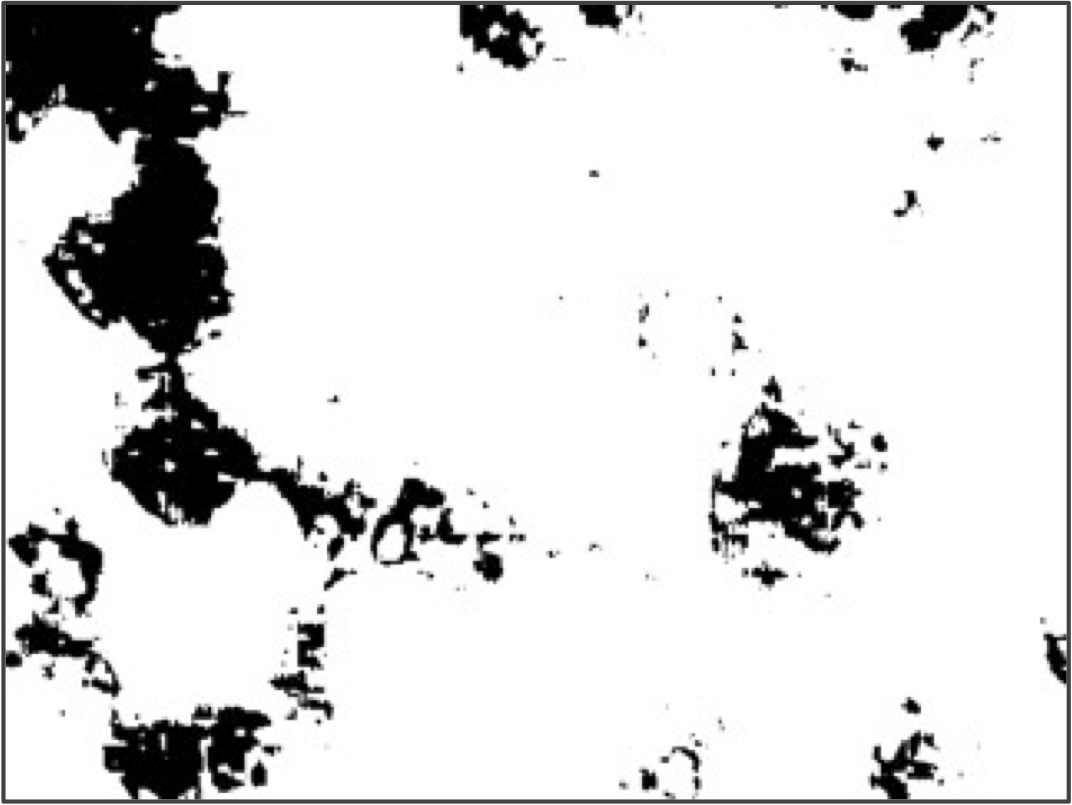
\includegraphics[width = 0.444\textwidth]{../images/neutrophil_binarized_blue.png}
\caption{A binarized version of the granulocyte from the previous figure (having image ID 3 in our dataset). A pixel is colored white if it has a blue value of 153 or greater, and the pixel is colored black otherwise. The region with the nucleus is not clearly visible because much of the background of the image, which is very light, also has a high blue value.}
\label{fig:neutrophil_binarized_blue}
\end{figure}

\begin{qbox}[%
How might we modify our segmentation approach to perform a binarization that identifies the WBC nucleus more effectively?
]\end{qbox}


We were unable to distinguish between the image background and the WBC nucleus using blue color values, but a color picker verifies that WBC nuclear pixels have a green content that is much lower than the background and a red content that is lower than every other part of the image. \autoref{fig:neutrophil_binarized_other_colors} shows two binarizations of the original image using a green threshold of 153 and a red threshold of 166.

\begin{figure}[p]
\centering
\tabcolsep = 2.5em
\mySfFamily
 FILL IN TWO IMAGES

\caption{Two more binarized versions of the neutrophil image from the figure above, based on the green and red channels. For both of these colors, the WBC nucleus tends to have lower values than other parts of the original image. (Left) A binarization in which a pixel is turned white if it has a green value less than or equal to 153. (Right) A binarization in which a pixel is turned white if it has a red value less than or equal to 166.}
\label{fig:neutrophil_binarized_other_colors}
\end{figure}

It would seem that we should work with the binarized image based on the red threshold, which contains the clearest image of the nucleus among the three binarized images. However, note that each threshold was successful in eliminating some of the non-nuclear parts of the image. For example, consider the white blob in the top left of the binarized image based on the red threshold. (CITE FIGURE)

This insight gives us an idea: if each of the three images is successful at excluding some part of the image, then let us produce a fourth image such that a pixel is white if it is white in all three binarized images. In the following tutorial, we will build an R pipeline that implements this approach to produce binarized WBC nuclei for all our blood cell images.

TUTORIAL POINTER

\FloatBarrier
\phantomsection
\subsection{Successful segmentation is subject to parameters}

If we segment all of the images in the dataset via the same process, then we typically obtain a nice result, as indicated in \autoref{fig:segmentation} for the sample monocyte and lymphocyte images presented in the [introduction](home). Even though these images have been binarized, the large irregular shape of the monocyte nucleus and the small round shape of the lymphocyte nucleus are still visible.

\begin{figure}[h]
\centering
\tabcolsep = 2.5em
\mySfFamily
 FILL IN TWO IMAGES

\caption{Image segmentation of the monocyte (left) and lymphocyte (right) corresponding to IDs 15 and 20 in the provided dataset.}
\label{fig:segmentation}
\end{figure}

This is not to say that our segmentation pipeline is perfect. \autoref{fig:segmentation_imperfect} illustrates that for a few images in our dataset, we may not correctly segment the entire nucleus.

\begin{figure}[h]
\centering
\tabcolsep = 2.5em
\mySfFamily
 FILL IN TWO IMAGES

\caption{(Left) An image of a WBC (ID: 167). (Right) The binarization of this image, showing that the nucleus is not correctly identified during segmentation using the parameters described in this lesson}
\label{fig:segmentation_imperfect}
\end{figure}

We can continue to tweak threshold parameters, but our relatively simple algorithm has successfully segmented most of the WBC nuclei from our dataset. We are ready to move on to classifying WBC nuclei into families according to their shape.

\FloatBarrier
\phantomsection
\section{An Overview of Classification and k-Nearest Neighbors}
\label{sec:knn}


\phantomsection
\subsection{The classification problem}

Labeling images of WBCs according to their family is a specific instance of an ubiqitous problem in data science, in which we wish to classify each object in a given dataset into one of \textvar{k} classes.

In our ongoing example, the data are images of WBCs, and the classes are the three main families of WBCs (granulocytes, lymphocytes, and monocytes). To take a different example, our data could be tumor genomes sequenced from cancer patients, which we want to classify based on which therapeutic should be prescribed for the patient. Or the data may be the past sales behavior of shoppers, who we want to classify into two classes based on a prediction of whether they will buy a new product.

\FloatBarrier
\phantomsection
\subsection{The iris flower dataset}

A classical dataset commonly used for motivating classification is the \textdef{iris flower dataset}{iris flower dataset}{FILL IN}, which was compiled by Edgar Anderson, and which Ronald Fisher used in a seminal paper on classification in 1936. Anderson took measurements from 150 iris flowers, equally divided among three species (\autoref{fig:iris_flowers}).\\

\begin{figure}[h]
\centering
\tabcolsep = 2.5em
\mySfFamily
 FILL IN IMAGES

\caption{Representative images of the three species of iris included in Anderson's iris flower dataset. (Left) \textit{Iris setosa}. (Center)  \textit{Iris versicolor}. (Right) \textit{Iris virginica}. Image courtesies, from left to right: Emma Forsberg, unknown author, Robert H. Mohlenbrock.}
\label{fig:iris_flowers}
\end{figure}

Anderson measured four attributes, or \textdef{features}{features}{FILL IN}, of each of the flowers in his dataset: both the width and height of the flower's petal, and both the width and height of the flower's sepal (a green offshoot beneath the petals). The features and species labels for twelve of the flowers in the iris flower dataset are shown in \autoref{fig:iris_feature_table}. Fisher considered whether it was possible to classify each flower according to its species using only the features Anderson had measured.\\

\begin{figure}[h]
\centering
\tabcolsep = 2.5em
\mySfFamily
\begin{tabular}{c c c c c}
Sepal length (cm) & Sepal width (cm) & Petal length (cm) & Petal width (cm) & Species \\
5.1 & 3.5 & 1.4 & 0.2 & \textit{Iris setosa} \\
4.9 & 3.0 & 1.4 & 0.2 & \textit{Iris setosa} \\
4.7 & 3.2 & 1.3 & 0.2 & \textit{Iris setosa} \\
4.6 & 3.1 & 1.5 & 0.2 & \textit{Iris setosa} \\
7.0 & 3.2 & 4.7 & 1.4 & \textit{Iris versicolor} \\
6.4 & 3.2 & 4.5 & 1.5 & \textit{Iris versicolor} \\
6.9 & 3.1 & 4.9 & 1.5 & \textit{Iris versicolor} \\
5.5 & 2.3 & 4.0 & 1.3 & \textit{Iris versicolor} \\
6.3 & 3.3 & 6.0 & 2.5 & \textit{Iris virginica} \\
5.8 & 2.7 & 5.1 & 1.9 & \textit{Iris virginica} \\
7.1 & 3.0 & 5.9 & 2.1 & \textit{Iris virginica} \\
6.3 & 2.9 & 5.6 & 1.8 & \textit{Iris virginica} \\
\end{tabular}
\caption{A table containing values of the four features for twelve members of the iris flower dataset. The complete dataset was accessed from the University of California, Irvine Machine Learning Repository.}
\label{fig:iris_feature_table}
\end{figure}

\begin{qbox}[%
What characteristics do flowers from each species tend to share in terms of the four features in \autoref{fig:iris_feature_table}?
]\end{qbox}

\FloatBarrier
\phantomsection
\subsection{From flowers to vectors}

If we were to use only two features in the Iris flower dataset, then a flower's feature values \textvar{x} and \textvar{y} could be represented as a point in two-dimensional space $(x, y)$. \autoref{fig:iris_petal_data} shows such a plot for the features of petal length (x-axis) and petal width (y-axis).

\begin{figure}[h]
\centering
\mySfFamily
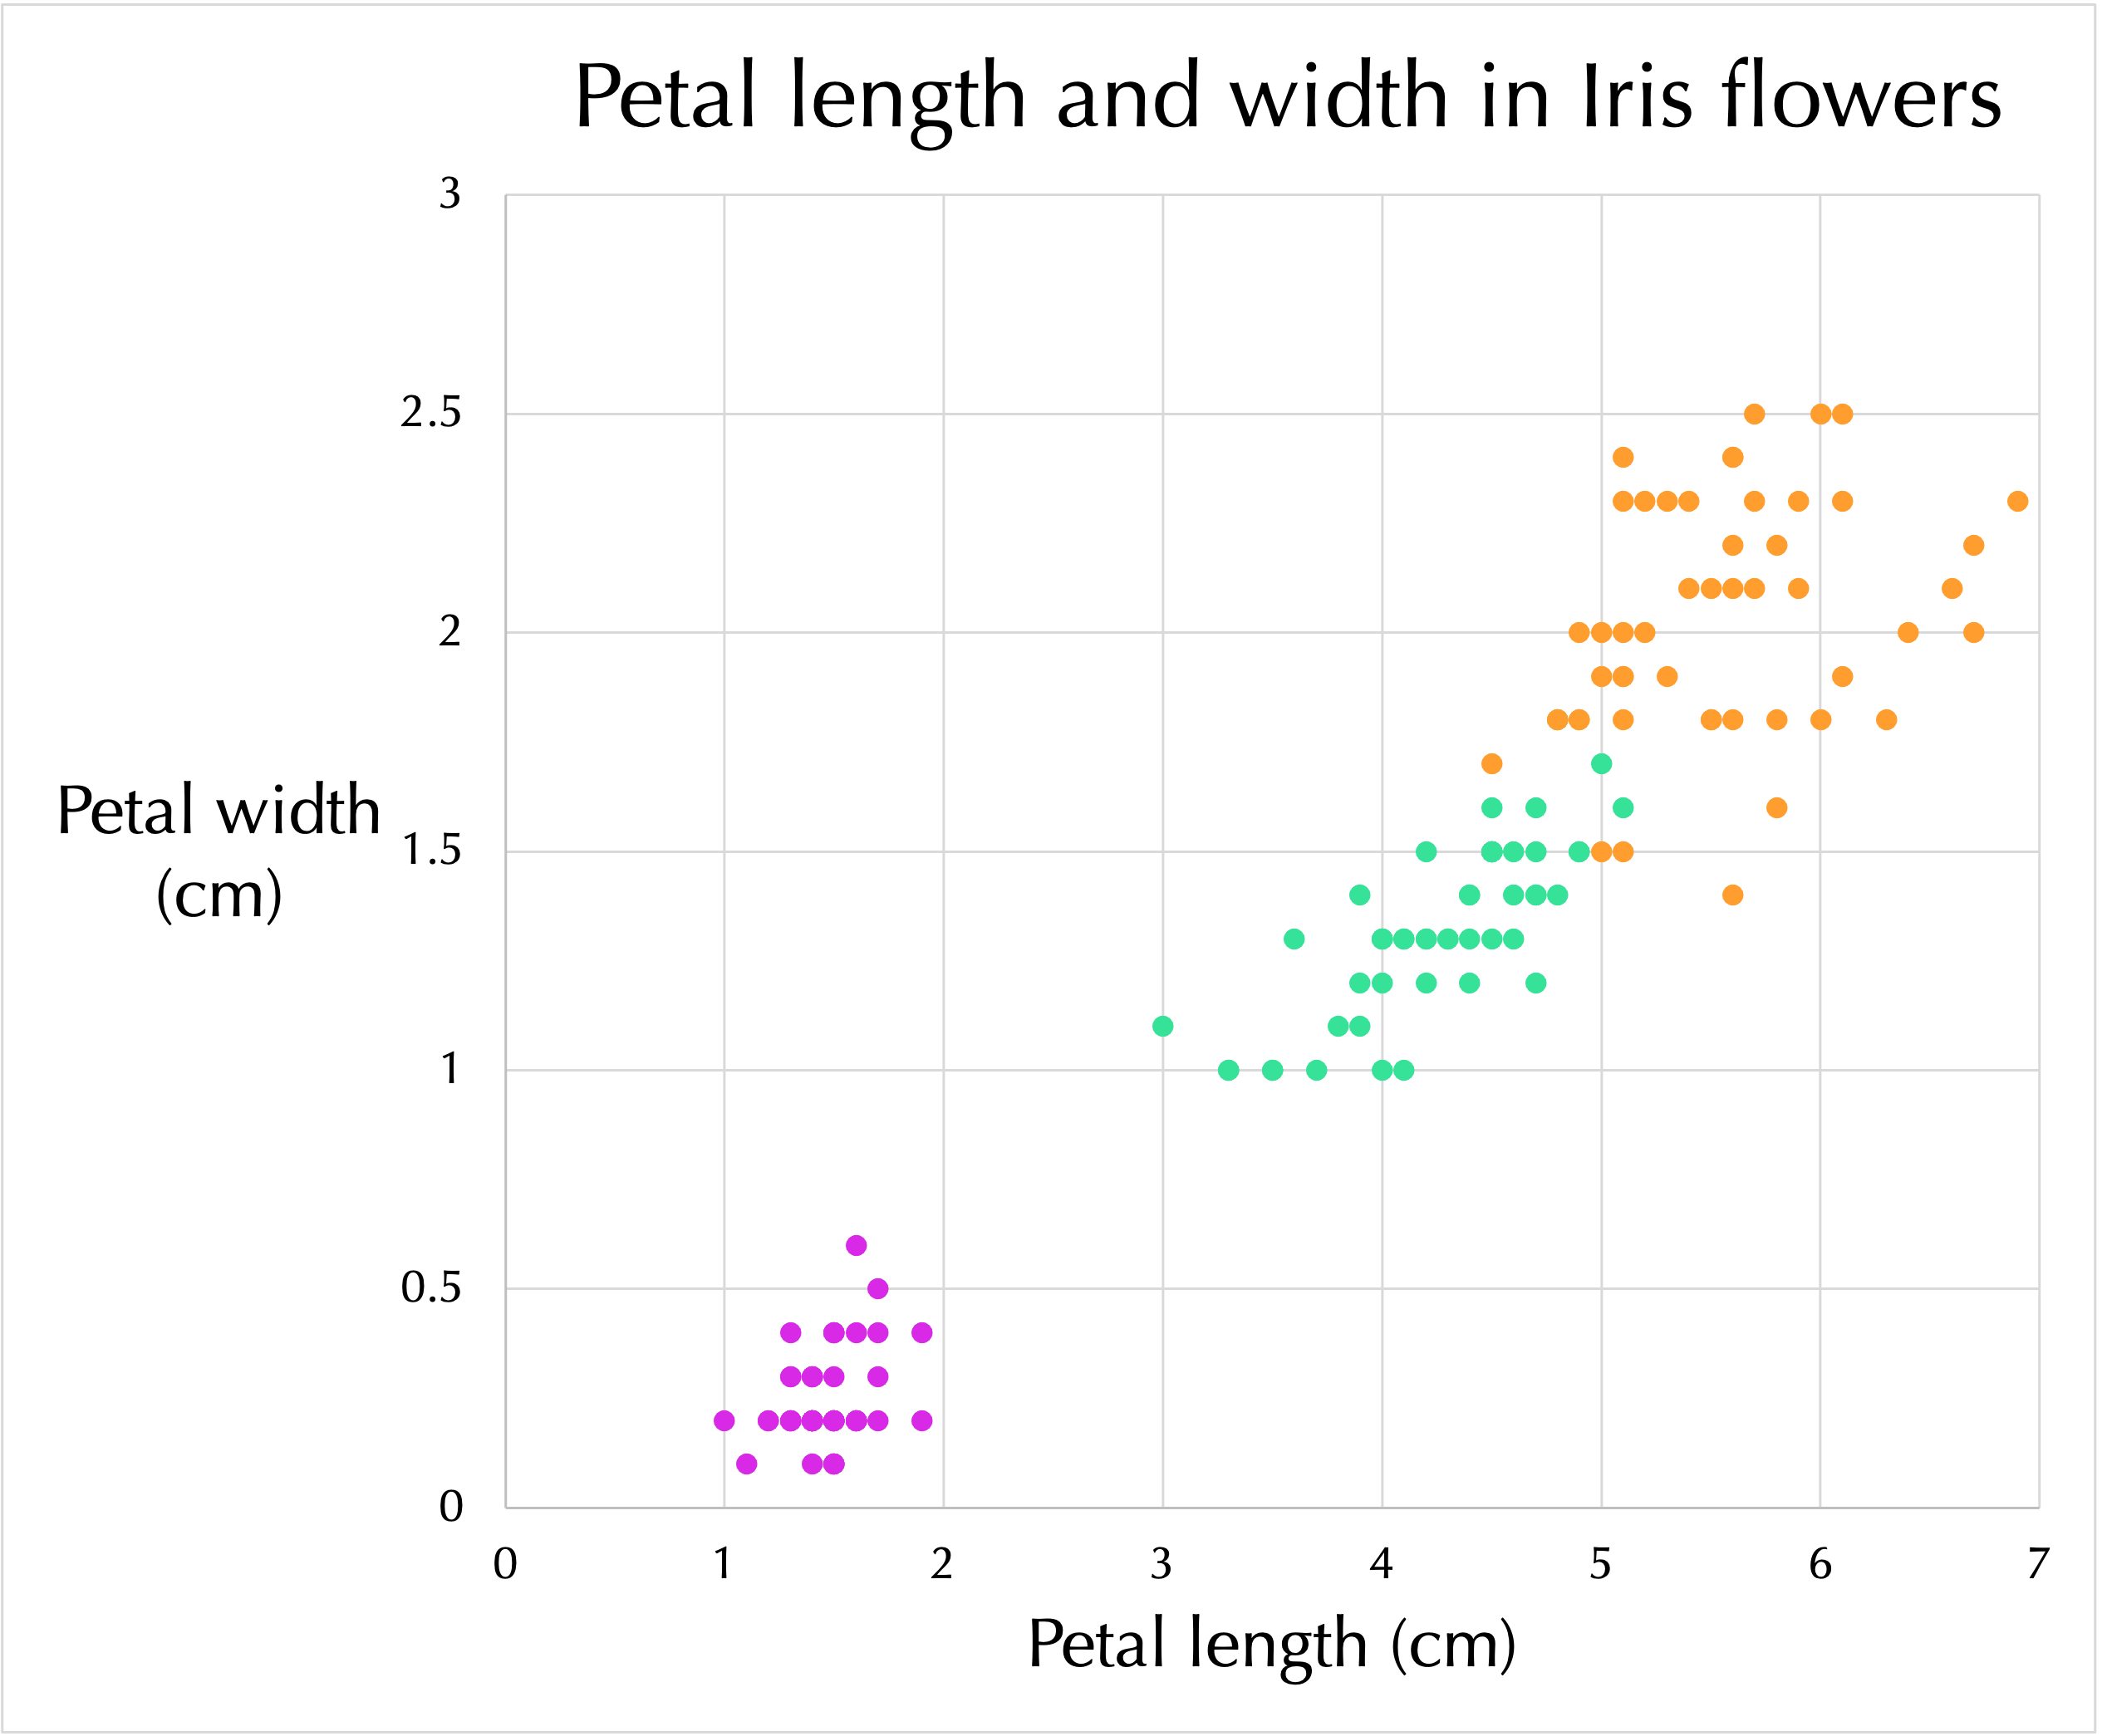
\includegraphics[width = 0.444\textwidth]{../images/iris_petal_data.png}
\caption{Petal width (x-axis) plotted against width (y-axis) for each of the flowers in the iris flower dataset, colored by species. There are not fifty points corresponding to every species because some flowers have the same petal length and width.}
\label{fig:iris_petal_data}
\end{figure}

Note how stark the pattern in \autoref{fig:iris_petal_data} is. Even though we chose only two features from the Iris flowers, the points associated with the flowers can be divided into three main clusters by species. In other words, nearby points tend to correspond to flowers from the same species.

If we were to use all four features for the iris dataset, then every flower would be represented by a point in four-dimensional space. For example, the first flower in our initial table of iris features would be represented by the point $(5.1, 3.5, 1.4, 0.2)$. In general, when classifying a collection of data with \textvar{n} features, each element in the dataset can be represented by a \textdef{feature vector}{feature vector}{FILL IN} of length \textvar{n}, whose \textvar{i}-th value corresponds to its value for the \textvar{i}-th feature.

\FloatBarrier
\phantomsection
\subsection{Classifying unknown elements with k-nearest neighbors}

For the iris flower dataset, recall our observation that data points were more likely to belong to the same class if they were nearby. Our hope is that this fact is true for other datasets, that elements from the same class will have feature vectors that are close in \textvar{n}-dimensional space. If so, then we can classify a data point whose class is \textit{unknown} by determining which data points with \textit{known} classification it is near.\\

\begin{qbox}[%
Consider the point with unknown class (gray) in \autoref{fig:knn_neighborhood}. Should it be assigned to the class of the green points or to the class of the blue points?
]\end{qbox}

\begin{figure}[h]
\centering
\mySfFamily
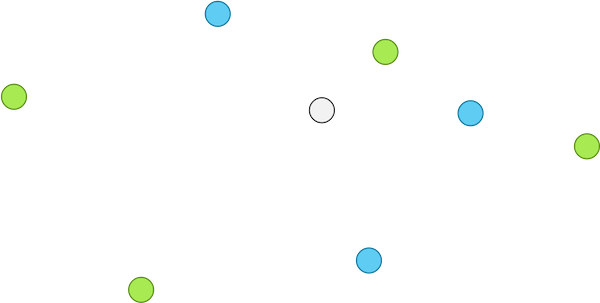
\includegraphics[width = 0.444\textwidth]{../images/knn_neighborhood.png}
\caption{An unknown point (gray) along with a collection of nearby points belonging to two classes, colored green and blue.}
\label{fig:knn_neighborhood}
\end{figure}

The preceding question indicates that classifying points can be surprisingly open-ended. Because of this freedom, researchers have devised a variety of different approaches for classifying data given data with known classes.

We will discuss a simple but powerful classification algorithm called \textdef{k-nearest neighbors (k-NN)}{k-nearest neighbors (k-NN)}{FILL IN}. In k-NN, we fix a positive integer \textvar{k} in advance, which will be used for classification of all points. Then, for each point with unknown class, we assign it the class possessed by the largest number of its \textvar{k} closest neighbors.

In the ongoing example, if we were using \textvar{k} equal to 1, then we would assign the unknown point from \autoref{fig:knn_neighborhood} to the green class (\autoref{fig:knn_neighborhood_k=1}).\\

\begin{figure}[h]
\centering
\mySfFamily
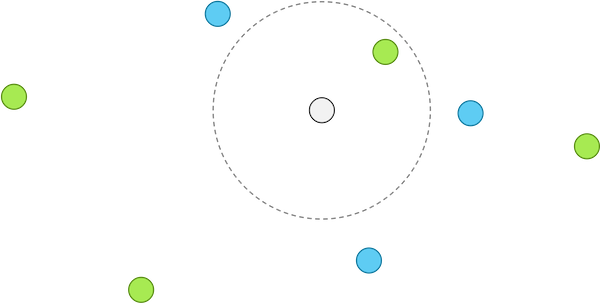
\includegraphics[width = 0.444\textwidth]{../images/knn_neighborhood_k=1.png}
\caption{When using k-NN with \textvar{k} equal to 1, we classify an unknown point according to the point of known class that is nearest; for this reason, the unknown point above would be assigned to the green class.}
\label{fig:knn_neighborhood_k=1}
\end{figure}

However, with the same data and \textvar{k} equal to 4, \autoref{fig:knn_neighborhood_k=4} shows that a majority of the \textvar{k} nearest neighbors are blue, and so we classify the unknown point as blue. This example reinforces a theme of this course, that the results of an algorithm can be sensitive to our choice of parameters.\\

\begin{figure}[h]
\centering
\mySfFamily
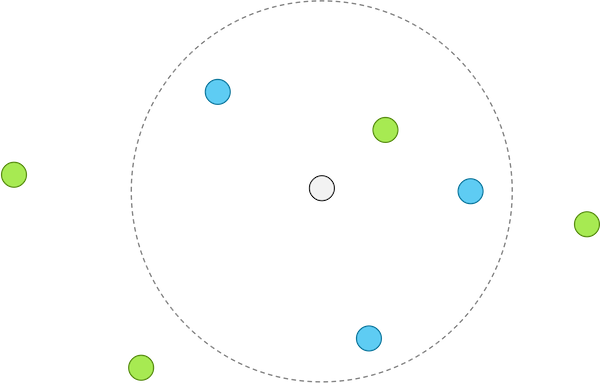
\includegraphics[width = 0.444\textwidth]{../images/knn_neighborhood_k=4.png}
\caption{When using k-NN with \textvar{k} equal to 4, k-NN will classify the unknown point as blue, since three of its four closest neighbors are blue.}
\label{fig:knn_neighborhood_k=4}
\end{figure}

\begin{qbox}[%
When \textvar{k} = 2 or \textvar{k} = 6 for the classification of the point in \autoref{fig:knn_neighborhood}, note that we obtain a tie in the number of points from each known class belonging to the \textvar{k} nearest neighbors of a point with unknown class. How could we break ties in k-NN?
]\end{qbox}

In the more general case in which feature vectors have length \textvar{n}, we can determine which points are nearest to a given point by using the \textdef{Euclidean distance}{Euclidean distance}{FILL IN}, which generalizes the distance between two points in two-dimensional space to vectors in \textvar{n}-dimensional space. Say that we have the vectors $x = (x_1, x_2, \ldots, x_n)$ and $y = (y_1, y_2, \ldots, y_n)$. Then the Euclidean distance between them is given by the sum of squares of differences between corresponding vector elements:

$$d(x, y) = \sqrt{(x_1 - y_1)^2 + (x_2 - y_2)^2 + \cdots + (x_n-y_n)^2}$$

We now have learned how to use k-NN to classify feature vectors with unknown classes given vectors with known classes. There is just one problem: how can we convert an image of a WBC into a vector?